\subsection{Gestione della configurazione}
\label{subsec:gestione_della_configurazione}
Il processo di gestione della configurazione si occupa di applicare procedure amministrative e tecniche durante tutto il ciclo di vita del software. 
In particolare identifica e definisce gli elementi software di un sistema per tenere traccia: delle modifiche, dello stato e dei rilasci dei file.
Inoltre garantisce la completezza, la coerenza e la correttezza degli elementi che compongono il prodotto software.

\subsubsection{Repository}
\label{subsubsec:repository}
I prodotti del progetto vengono memorizzati in più \glossario{repository}.
Di seguito vengono elencati i repository utilizzati dal gruppo, le loro caratteristiche e la loro struttura.

\paragraph{SorgentiDocumentazione}
Questo repository contiene i sorgenti della documentazione scritti usando il \hyperref[par:latex]{linguaggio LaTeX}.
Il repository segue la struttura indicata in \hyperref[fig:repo_sorgenti_documenti]{Figura \ref{fig:repo_sorgenti_documenti}}.
\begin{figure}[H]
    \dirtree{%
        .1 SorgentiDocumentazione.
            .2 .github.
                .3 DizionariLatex.
                    .4 \texttt{<dizionari>}
                .3 workflows.
                    .4 \texttt{<file worflows>}.
            .2 Candidatura.
            .2 RTB.
            .2 Packages.
            .2 Immagini.
            .2 \texttt{README.md}.
            .2 \texttt{.gitignore}.
    }
    \caption{Struttura repository SorgentiDocumentazione.}
    \label{fig:repo_sorgenti_documenti}
\end{figure}
Dove:
\begin{enumerate}
    \item \texttt{Candidatura}, \texttt{RTB} e \texttt{Packages} sono delle cartelle il cui contenuto viene spiegato nelle successive sezioni.
    \item \texttt{<file workflows>} sono dei file che definiscono le automazioni associate al repository e vengono denominati usando la sintassi \glossario{Pascal case}.
    \item \texttt{Immagini} è una cartella che contiene il logo del gruppo.
    \item \texttt{README.md} è un file che contiene la descrizione del repository e del gruppo.
    \item \texttt{.gitignore} è un file speciale che contiene una lista di file che il sistema di versionamento deve ignorare.
\end{enumerate}

\subparagraph{Candidatura}
La cartella candidatura ha la struttura indicata in \hyperref[fig:repo_sorgenti_documenti_candidatura]{Figura \ref{fig:repo_sorgenti_documenti_candidatura}}.
\begin{figure}[H]
    \dirtree{%
        .1 Candidatura.
            .2 VerbaliEsterni.
                .3 \texttt{<verbali esterni esplicativi>}.
            .2 VerbaliInterni.
                .3 \texttt{<verbali interni>}.
            .2 \texttt{<lettera di candidatura>}.
            .2 \texttt{<preventivo dei costi assunzione impegni>}.
            .2 \texttt{<valutazione capitolati>}.
    }
    \caption{Struttura cartella Candidatura.}
    \label{fig:repo_sorgenti_documenti_candidatura}
\end{figure}

\subparagraph{RTB}
La cartella RTB ha la struttura indicata in \hyperref[fig:repo_sorgenti_documenti_RTB]{Figura \ref{fig:repo_sorgenti_documenti_RTB}}.
\begin{figure}[H]
    \dirtree{%
        .1 RTB.
            .2 DocumentiInterni.
                .3 \texttt{<norme di progetto>}.
                .3 VerbaliInterni.
                .4 \texttt{<verbali interni>}.
            .2 DocumentiEsterni.
                .3 \texttt{<piano di progetto>}.
                .3 \texttt{<analisi dei requisiti>}.
                .3 VerbaliEsterni.
                    .4 \texttt{<verbali esterni>}.
    }
    \caption{Struttura cartella RTB.}
    \label{fig:repo_sorgenti_documenti_RTB}
\end{figure}

\subsubsection{Identificazione configuration item}
\label{subsubsec:identificazione_CI}
Di seguito vengono elencate le regole usate per nominare i \glossario{configuration item} elencati nella sezione \hyperref[subsubsec:repository]{repository}.
I file che non riguardano direttamente il progetto non vengono spiegati ulteriormente. 

\paragraph{Sorgenti documenti}
\begin{table}[H]
    \resizebox{\textwidth}{!}{
    \begin{tabular}{| c | c | c |}
        \hline
        \textbf{Nome} & \textbf{Identificativo} & \textbf{Registro modifiche} \\
        \hline 
        verbali interni & \texttt{<data>-<versione>} & sì \\
        \hline
        verbali esterni & \texttt{<data>-<versione>} & sì\\
        \hline
        verbali esterni esplicativi & \texttt{<data>-<proponente>-<versione>} & sì\\
        \hline
        lettera di candidatura & \texttt{LetteraDiCandidatura} & no\\
        \hline
        valutazione dei capitolati & \texttt{ValutazioneDeiCapitolati-<versione>} & sì\\
        \hline
        preventivo dei costi e assunzione impegni & \texttt{CostiImpegni-<versione>} & sì\\
        \hline
        piano di progetto & \texttt{PianoDiProgetto-<versione>} & sì\\
        \hline
        norme di progetto & \texttt{NormeDiProgetto-<versione>} & sì\\
        \hline
        Piano di qualifica & \texttt{PianoDiQualifica-<versione>} & sì\\
        \hline
        analisi dei requisiti & \texttt{AnalisiDeiRequisiti-<versione>} & sì\\
        \hline
    \end{tabular}}
    \caption{Configuration item del repository SorgentiDocumentazione.}
\end{table}
\noindent Dove:
\begin{itemize}
    \item Le date seguono lo schema \texttt{aaaa\_mm\_gg}.
    \item Il nome della proponente segue la sintassi \glossario{Pascal case}.
    \item Le versioni seguono lo schema indicato alla sezione \hyperref[par:versione_documenti]{Versione dei documenti}.
\end{itemize}
Il motivo dell'utilizzo di data e proponente all'interno dei nomi di alcune tipologie di documenti è che permettono un ordinamento sensato degli stessi.

\subsubsection{Controllo di versione}
Di seguito vengono riportati i metodi usati dal gruppo per tenere traccia delle versioni dei file contenuti nei repository.

\paragraph{Software di controllo di versione}
Il gruppo ha deciso di utilizzare Git come software per il controllo di versione.
I motivi di questa scelta sono:
\begin{enumerate}
    \item Git è abbastanza conosciuto dai membri del gruppo.
    \item Git è molto usato e quindi una conoscenza approfondita dello stesso è molto utile.
\end{enumerate}
Di seguito vengono fornite delle informazioni teoriche sulle scelte fatte dal gruppo sulla gestione del repository.
La separazione netta tra concetti teorici e pratici pur essendo "fastidiosa" per il lettore permette la modularità degli strumenti usati.

\subparagraph{Strategia di branching}
\label{subpar:strategia_di_branching_documenti}
Come \glossario{strategia di branching} il gruppo ha scelto l'utilizzo di Gitflow dato che permette di massimizzare il lavoro parallelo riducendo la complessità di risoluzione dei conflitti.
In \hyperref[fig:gitflow]{Figura \ref{fig:gitflow}} viene mostrato un esempio di utilizzo della strategia di branching Gitflow.
\begin{figure}[H]
    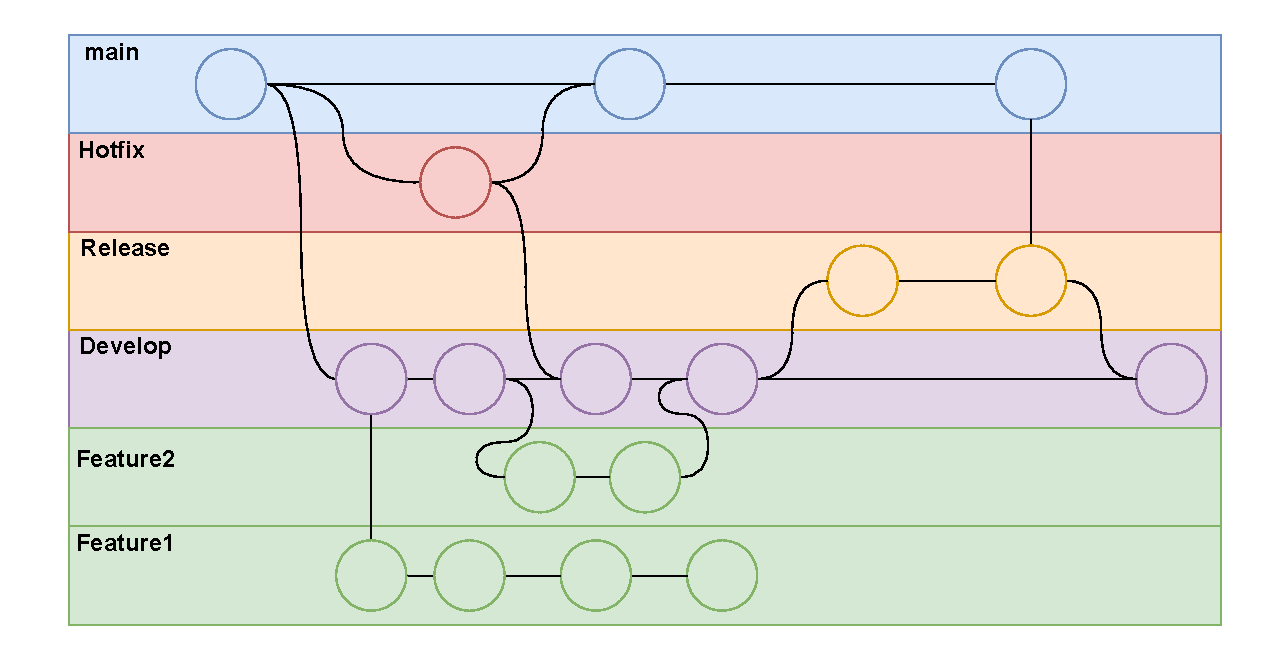
\includegraphics[scale=0.65]{Sezioni/ProcessiDiSupporto/Immagini/gitflow.pdf}
    \caption{Gitflow in azione(i cerchi sono commit e le linee i collegamenti tra essi)}
    \label{fig:gitflow}
\end{figure}
Di seguito vengono descritti i rami utilizzati da Gitflow e le convenzioni usate dal gruppo.
\begin{enumerate}

\item \textbf{main}

Il ramo \texttt{main} contiene la codeline principale ovvero le versioni dei file che compongono l'ultima baseline raggiunta.
Questo ramo è un ramo "stabile" nel senso che persiste nel repository lungo tutta la sua vita.

\item \textbf{develop}

Il ramo \texttt{develop} contiene la codeline secondaria ovvero i cambiamenti verificati che si sommeranno formando la prossima baseline.
Anche questo ramo è un ramo "stabile" e viene creato a partire dal ramo \texttt{main}.

\item \textbf{feature}
\label{item:rami_feature}
I rami \texttt{feature} vengono usati dai membri del gruppo per implementare le modifiche.
Sono dei rami "provvisori" nel senso che esistono finché il loro contenuto non viene verificato.
I rami \texttt{feature} vengono creati a partire dal ramo \texttt{develop} e confluiscono in esso quando il loro contenuto passa con successo la verifica.
Il gruppo ha deciso di utilizzare la seguente convenzione per la denominazione di questi rami:
\begin{lstlisting}
    feature/#<idRichiestaDiModifica>
\end{lstlisting}
Così facendo si ottiene un collegamento immediato tra ramo di \texttt{feature} e richiesta di modifica.

\item \textbf{hotfix}

I rami \texttt{hotfix} vengono usati per eseguire modifiche rapide e di dimensioni ridotte.
Queste modifiche non influenzano quindi le versioni dei documenti.
Questi rami sono "provvisori" nel senso che vengono eliminati dopo che le loro modifiche sono state allineate ai rami \texttt{main} e \texttt{develop}.


\item \textbf{release}

I rami \texttt{release} vengono usati dal Responsabile del gruppo per approvare il contenuto del ramo \texttt{develop} consolidandolo in una baseline nella codeline principale.
Sono dei rami "provvisori" nel senso che esistono finché il loro contenuto non viene approvato.
I rami \texttt{release} vengono creati a partire dal ramo \texttt{develop} e confluiscono nei rami \texttt{main} e \texttt{develop}.
Il gruppo ha deciso di utilizzare la seguente convenzione per la denominazione di questi rami:
\begin{lstlisting}
    feature/nomeMilestone
\end{lstlisting}
Così facendo si ottiene un collegamento immediato tra ramo di \texttt{release} e la milestone che raggiunge.
\end{enumerate}

\subparagraph{Risoluzione dei conflitti}
\label{subpar:risoluzione_dei_conflitti}
Utilizzando Gitflow i conflitti possono presentarsi nelle seguenti fusioni(merge) di rami(indicate come "partenza \textrightarrow\ destinazione"):
\begin{enumerate}
    \item \textbf{release} \textrightarrow\ \textbf{main}
    
    I conflitti si presentano quando nel ramo di \texttt{release} esistono modifiche su uno o più file presenti nel ramo \texttt{main}.
    In questo caso il contenuto del ramo \texttt{release} ha la precedenza dato che è più aggiornato.
    
    \item \textbf{hotfix} \textrightarrow\ \textbf{develop}
    
    I conflitti si presentano quando la correzione rapida eseguita nel ramo \texttt{hotfix} riguarda uno o più file che nel mentre sono stati modificati nel ramo \texttt{develop}.
    In questo caso è importante che le correzioni del ramo \texttt{hotfix} persistano nel ramo \texttt{develop} dopo la fusione.
    Il ramo \texttt{hotfix} ha quindi la precedenza.   


    \item \textbf{feature} \textrightarrow\ \textbf{develop}
   
    I conflitti possono presentarsi se due membri del gruppo lavorano sullo stesso documento allo stesso tempo.
    In questo caso entrambe le modifiche verificate devono raggiungere il ramo \texttt{develop}.
    Bisogna però porre attenzione a mantenere il corretto ordine del \hyperref[par:registro_delle_modifiche]{Registro delle modifiche}.
\end{enumerate}


\paragraph{Registro delle modifiche}
\label{par:registro_delle_modifiche}
Oltre all'utilizzo di un software di controllo di versione il gruppo ha deciso di dotare alcuni documenti di una tabella chiamata registro delle modifiche.
Tale tabella se il repository fosse gestito in modo impeccabile sarebbe una copia dei dati già registrati nella stessa.
Tuttavia il metodo di lavoro del gruppo è in continua evoluzione quindi possono accadere modifiche distruttive che eliminano le versioni dei configuration item apperteneti alla baseline precedente.
Il registro delle modifiche è quindi uno strumento a supporto del controllo di configurazione ed è più "attendibile" rispetto alla storia del repository Git.
I documenti per cui viene usato il registro delle modifiche sono indicati nella sezione \hyperref[subsubsec:identificazione_CI]{Identificazione configuration item}.

Di seguito viene indicata la struttura del registro delle modifiche:
\begin{enumerate}
    \item \textbf{Versione}: versione del documento dopo la verifica della modifica.
    \item \textbf{Data}: data in cui è avvenuta la modifica.
    \item \textbf{Autore/i}: nome e cognome dei componenti del gruppo che hanno eseguito le modifiche.
    \item \textbf{Verificatore/i}: nome e cognome dei verificatori.
    \item \textbf{Descrizione}: breve descrizione delle modifiche indicando un link alle sezioni modificate.
    
    La descrizione permette ai membri del team di capire velocemente la necessità di allinearsi a nuove informazioni. 
\end{enumerate} 
\textbf{Nota bene}: Le righe del registro delle modifiche sono ordinate per versione decrescente.

\paragraph{Versione}
\label{par:versione_documenti}
Le versioni dei documenti vengono indicate seguendo lo schema di versionamento:
\begin{lstlisting}
    vX.Y
\end{lstlisting}
Dove:
\begin{enumerate}
    \item \texttt{X}: intero positivo che indica la versione major del documento.
    La versione major indica a quante volte il documento ha raggiunto uno stato ritenuto come "stabile" dal gruppo.

    \item \texttt{Y}: intero positivo che indica la versione minor del documento.
    La versione minor indica il numero di modifiche effettuate al documento a seguito dell'ultima versione major.
\end{enumerate}
Uno schema di versionamento a due valori risulta più semplice dato che si concentra solo sulle modifiche significative in termini di contenuto dei documenti.

\textbf{Nota bene}: per evitare ambiguità con le estensioni dei documenti il gruppo ha deciso di rappresentare la versione nei nomi dei documenti usando la notazione \texttt{vX\_Y}.

\subsubsection{Gestione delle modifiche}
Una modifica è intesa come un azione che ha lo scopo di modificare lo stato di uno o più file appartenenti all'ultima baseline raggiunta in un repository. 

\paragraph{Richieste di modifica}
Ogni modifica deve essere preceduta da una richiesta di modifica che deve essere discussa e accettata tramite votazione di maggioranza.
Le richieste di modifica vengono registrate e gestite utilizzando il servizio di issue tracking offerto da GitHub.  
Le informazioni tecniche riguardanti la gestione delle issue vengono indicate alla sezione \hyperref[subpar:ITS]{Issue Tracking System}.
Una richiesta di modifica deve contenere le seguenti informazioni:
\begin{itemize}
    \item \textbf{Nome del file da modificare}: indicandone il percorso all'interno del repository.
    \item \textbf{Data della richiesta}.
    \item \textbf{Tempo stimato per implementare il cambiamento}: indicata nel piano di progetto nella pianificazione dello sprint attuale.
    \item \textbf{Tipo di modifica}.
    \item \textbf{Descrizione della modifica da fare}.
    \item \textbf{Stato}: indica lo stato della richiesta al momento e permette al gruppo di capire cosa fare.
\end{itemize}

\subparagraph{Descrizione modifica}
La descrizione di una modifica deve essere rappresentata tramite un check list contenente i compiti da svolgere per implementare la modifica.
Questo permette:
\begin{enumerate}
    \item [a.] A chi implementa la modifica di avere una linea guida su cosa fare anche dopo tanto tempo rispetto alla discussione della modifica nel gruppo.
    \item [b.] A chi verifica la modifica di sapere che cosa doveva essere fatto.
\end{enumerate} 

\paragraph{Ciclo di vita delle richieste di modifica}
\label{par:ciclo_vita_richieste_di_modifica}
Gli stati che una richiesta di modifica attraversa durante il suo ciclo di vita sono riassunti nel diagramma in \hyperref[fig:ciclo_di_vita_modifiche_documenti]{Figura \ref{fig:ciclo_di_vita_modifiche_documenti}}.
\begin{figure}[h!]
    \center
    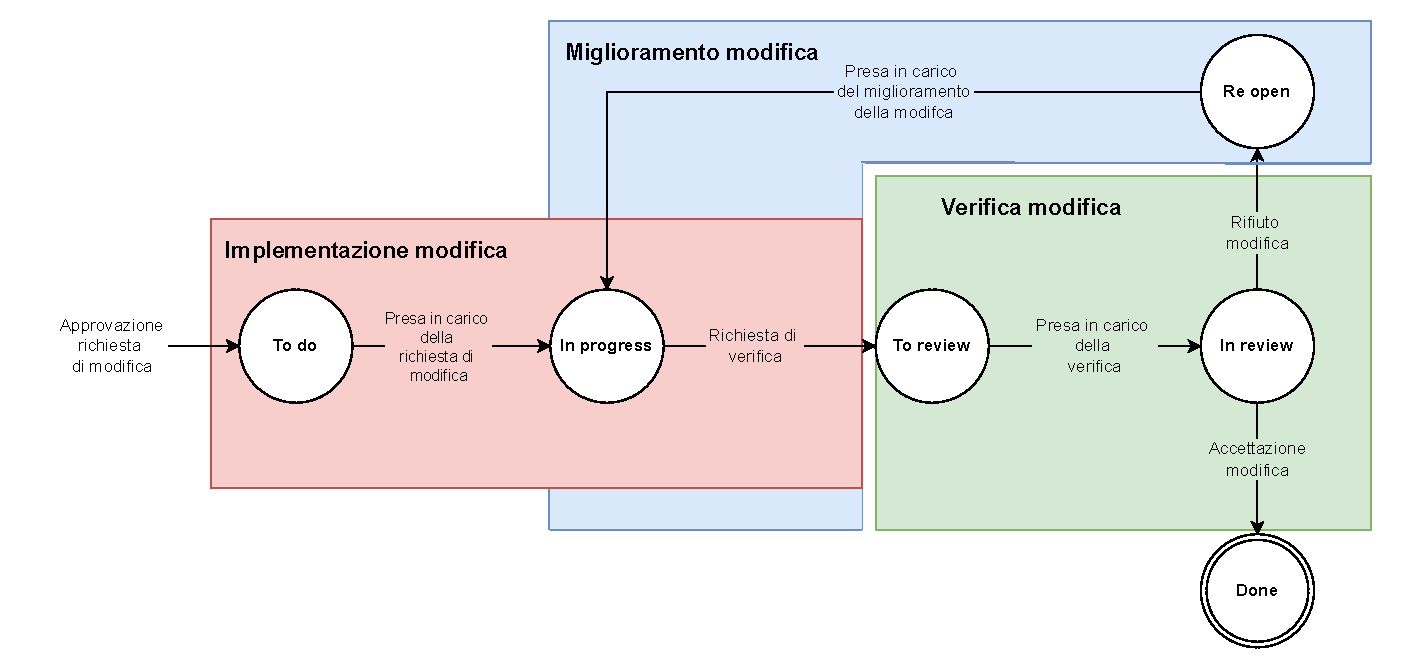
\includegraphics[scale=0.6]{Sezioni/ProcessiDiSupporto/Immagini/lifecycle_modifica.pdf}
    \caption{Ciclo di vita di una richiesta di modifica}
    \label{fig:ciclo_di_vita_modifiche_documenti}
\end{figure}

\paragraph{Stati}\label{par:stati}
In particolare gli stati di una richiesta di modifica sono:
\begin{enumerate}
    \item \textbf{To do}: la richiesta di modifica è stata approvata dal gruppo, registrata in GitHub e appartiene ai compiti che portano al raggiungimento di una prossima baseline.
    \item \textbf{In progress}: la richiesta di modifica è stata presa in carico da un membro del gruppo.
    \item \textbf{To review}: la modifica è stata implementata dal membro del gruppo che la presa in carico.
    Prima di contribuire alla prossima baseline deve essere verificata.
    \item \textbf{In review}: un Verificatore sta procedendo a eseguire la verifica della modifica.
    \item \textbf{Re open}: la modifica non è stata accettata dal Verificatore e deve quindi essere migliorata.
    \item \textbf{Done}: la modifica è stata accettata dal Verificatore e quindi è stata integrata nella prossima baseline. 
\end{enumerate}

\paragraph{Cambiamenti di stato}
I cambiamenti di stato di una richiesta di modifica durante al suo ciclo di vita sono:
\begin{enumerate}
    \item \textbf{Presa in carico della richiesta di modifica}(\textbf{To do} \textrightarrow\ \textbf{In progress})
    
    Avviene manualmente seguendo la procedura a carico del modificatore indicata alla sezione \hyperref[subpar:presa_carico_modifica]{Presa in carico di una modifica}.
    
    \item \textbf{Richiesta di verifica}(\textbf{In progress} \textrightarrow\ \textbf{To review})
    
    Avviene manualmente seguendo la procedura a carico del modificatore indicata alla sezione \hyperref[subpar:github_richiesta_di_verifica]{Richiesta di verifica}.
    
    \item \textbf{Presa in carico della verifica}(\textbf{To review} \textrightarrow\ \textbf{In review})
    
    Avviene manualmente seguendo la procedura indicata alla sezione \hyperref[subpar:presa_carico_verifica]{Presa in carico di una verifica}.
    
    \item  \textbf{Rifiuto modifica}(\textbf{In review} \textrightarrow\ \textbf{Re open})
    
    Avviene in automatico nel caso in cui la verifica della modifica abbia esito negativo.
    
    \item \textbf{Accettazione modifica}(\textbf{In review} \textrightarrow\ \textbf{Done})
    
    Avviene in automatico nel caso in cui la verifica della modifica abbia esito positivo.
    
    \item \textbf{Presa in carcio del migliroamento della modifica}(\textbf{Re open} \textrightarrow\ \textbf{In progress})
    
    Avviene manualmente seguendo la procedura a carico del modificatore indicata alla sezione \hyperref[subpar:presa_carico_modifica]{Presa in carico di una modifica}.
\end{enumerate}

\paragraph{Fasi}
Le fasi del ciclo di vita di una modifica sono:
\begin{enumerate}
    \item \textbf{Implementazione modifica}: comprende gli stati "To do", "In progress", "To review" e le transizioni tra gli stessi.

    \item \textbf{Verifica modifica}: comprende gli stati "To review", "In review", "Done", "Re open" e le transizioni tra gli stessi.
    
  
    \item \textbf{Miglioramento modifica}: comprende gli stati "Re open", "In progress", "To review" e le transizioni tra gli stessi. 
  
\end{enumerate}

\subparagraph{Implementazione modifica}
Per implementare una modifica è necessario eseguire i seguenti passi:
\begin{enumerate}
\item \hyperref[subpar:presa_carico_modifica]{Presa in carico della modifica}.

\item \hyperref[subpar:pull]{Pull ramo} \texttt{develop}.

\item \hyperref[subpar:branch]{Creazione ramo} \texttt{feature}(vedere \hyperref[item:rami_feature]{rami feature}).

\item Colmare la necessità della richiesta di cambiamento assicurandosi di soddisfare la check list.
Questa operazione deve avvenire seguendo il processo che regola l'implementazione della tipologia di file da modificare.

\textbf{Nota bene}: Per alcuni documenti è necessario aggiungere al \hyperref[par:registro_delle_modifiche]{registro delle modifiche} una nuova riga contenente le informazioni per le colonne "Autore/i" e "Descrizione". 

\item \hyperref[subpar:commit]{Commit} delle modifiche nel ramo \texttt{feature}.

\item \hyperref[subpar:push]{Push ramo} \texttt{feature}.

\item \hyperref[subpar:github_richiesta_di_verifica]{Richiesta di verifica} aggiungendo nel primo commento della
 pull request i seguenti campi:
 \begin{enumerate}
    \item closes \#\textless ID della issue che richiede la verifica\textgreater
    \item Tempo impiegato: \textless numero delle ore effettive usate per svolgere la issue\textgreater
 \end{enumerate}

\end{enumerate}

\subparagraph{Verifica modifica}
Per verificare un cambiamento è necessario eseguire i seguenti passi:
\begin{enumerate}
    \item \hyperref[subpar:presa_carico_verifica]{Presa in carico della verifica}.
    
    \item \hyperref[subpar:pull]{Pull} ramo \texttt{feature}(vedere \hyperref[item:rami_feature]{rami feature}).
    
    \item Verificare i cambiamenti seguendo le regole indicate nella sezione \hyperref[]{Verifica}.
    
    \textbf{Nota bene}: Nel caso di rifiuto per alcuni documenti è necessario aggiornare l'ultima riga del \hyperref[par:registro_delle_modifiche]{Registro delle modifiche} specificando la colonna "Verificatore/i".

    Nel caso di accettazione oltre a fare ciò è necessario specificare la colonna "Versione" e aggiornare la versione mostrata nel documento(leggere sezione \hyperref[par:struttura_di_base_documenti]{Struttura di base dei documenti}).

    \item \hyperref[subpar:commit]{Commit} delle modifiche sul ramo \texttt{feature}.
    
    \item \hyperref[subpar:push]{Push} del ramo \texttt{feature}.

    \item \hyperref[subpar:accettazione_modifiche]{Accettazione} o \hyperref[subpar:rifiuto_modifiche]{rifiuto} delle modifiche.
\end{enumerate}

\subparagraph{Miglioramento modifica}
  
Per eseguire il miglioramento di una modifica è necessario eseguire i seguenti passi:
\begin{enumerate}
\item \hyperref[subpar:presa_carico_modifica]{Presa in carico del miglioramento}.

\item \hyperref[subpar:pull]{Pull} branch \texttt{feature}(vedere \hyperref[item:rami_feature]{rami feature}).

\item Modificare il documento assicurandosi di soddisfare la check list e le informazioni aggiuntive date dal verificatore che ha rifiutato la modifica.
Questa operazione deve avvenire seguendo il processo che regola l'implementazione della tipologia di configuration item.

\textbf{Nota bene}: Per alcuni documenti è necessario aggiungere all'ultima riga del \hyperref[par:registro_delle_modifiche]{registro delle modifiche} le informazioni per la colonna "Autore/i". 

\item \hyperref[subpar:commit]{Commit} delle modifiche nel ramo \texttt{feature}.

\item \hyperref[subpar:push]{Push} ramo \texttt{feature}.

\item \hyperref[subpar:github_richiesta_di_verifica]{Richiesta di verifica}.
\end{enumerate}

\subsubsection{Approvazione}
Di seguito viene documentata l'attività di approvazione delle versioni dei file che devono essere consolidate in una baseline.
L'approvazione deve essere eseguita dal Responsabile del gruppo di lavoro e prevede le seguenti operazioni:
\begin{enumerate}
    \item Creazione ramo \texttt{release} seguendo le regole indicate nella sezione \hyperref[subpar:strategia_di_branching_documenti]{Strategia di branching}.
    \item Eseguire eventuali modifiche correttive minori.
    
    \textbf{Nota bene}: Aggiungere una nuova riga nel registro delle modifiche indicando i valori per le colonne "Autore/i", "Versione" e "Data".
    Inoltre usare il valore "Approvazione modifiche" per la colonna "Descrizione".

    \item \hyperref[subpar:commit]{Commit} delle modifiche.
    \item \hyperref[subpar:merge]{Merge} del ramo \texttt{release} nel ramo \texttt{main} e nel ramo \texttt{develop} seguendo le regole indicate alla sezione \hyperref[subpar:risoluzione_dei_conflitti]{Risoluzione dei conflitti}.
    \item \hyperref[subpar:push]{push} dei rami \texttt{main} e \texttt{develop}.
\end{enumerate}

\subsubsection{Distribuzione dei documenti}
La distribuzione dei documenti avviene mediante l'utilizzo di un sito web disponibile al link \href{https://alt-f4-eng.github.io/Documentazione/}{https://alt-f4-eng.github.io/Documentazione/}.
I documenti distribuiti vengono aggiornati ogni volta che viene modificata la baseline ovvero ogni volta che viene modificato il ramo \texttt{main}.
L'aggiornamento dei documenti segue la procedura indicata alla sezione \hyperref[par:pubblicazione_documenti]{Pubblicazione dei documenti}